%%% The main file. It contains definitions of basic parameters and includes all other parts.

%% Settings for single-side (simplex) printing
% Margins: left 40mm, right 25mm, top and bottom 25mm
% (but beware, LaTeX adds 1in implicitly)
\documentclass[12pt,a4paper]{report}
\setlength\textwidth{145mm}
\setlength\textheight{247mm}
\setlength\oddsidemargin{15mm}
\setlength\evensidemargin{15mm}
\setlength\topmargin{0mm}
\setlength\headsep{0mm}
\setlength\headheight{0mm}
% \openright makes the following text appear on a right-hand page
\let\openright=\clearpage

%% Settings for two-sided (duplex) printing
% \documentclass[12pt,a4paper,twoside,openright]{report}
% \setlength\textwidth{145mm}
% \setlength\textheight{247mm}
% \setlength\oddsidemargin{14.2mm}
% \setlength\evensidemargin{0mm}
% \setlength\topmargin{0mm}
% \setlength\headsep{0mm}
% \setlength\headheight{0mm}
% \let\openright=\cleardoublepage

%% Generate PDF/A-2u
\usepackage[a-2u]{pdfx}

%% Character encoding: usually latin2, cp1250 or utf8:
\usepackage[utf8]{inputenc}

%% Prefer Latin Modern fonts
\usepackage{lmodern}

%% Further useful packages (included in most LaTeX distributions)
\usepackage{amsmath}        % extensions for typesetting of math
\usepackage{amsfonts}       % math fonts
\usepackage{amsthm}         % theorems, definitions, etc.
\usepackage{bbding}         % various symbols (squares, asterisks, scissors, ...)
\usepackage{bm}             % boldface symbols (\bm)
\usepackage{graphicx}       % embedding of pictures
\usepackage{fancyvrb}       % improved verbatim environment
\usepackage{natbib}         % citation style AUTHOR (YEAR), or AUTHOR [NUMBER]
\usepackage[nottoc]{tocbibind} % makes sure that bibliography and the lists
			    % of figures/tables are included in the table
			    % of contents
\usepackage{dcolumn}        % improved alignment of table columns
\usepackage{booktabs}       % improved horizontal lines in tables
\usepackage{paralist}       % improved enumerate and itemize
\usepackage{xcolor}         % typesetting in color

\usepackage{hyperref}       % URL support
\usepackage{qtree}          % drawing trees

%%% Basic information on the thesis

% Thesis title in English (exactly as in the formal assignment)
\def\ThesisTitle{Board game with artificial intelligence}

% Author of the thesis
\def\ThesisAuthor{Daniel Crha}

% Year when the thesis is submitted
\def\YearSubmitted{2020}

% Name of the department or institute, where the work was officially assigned
% (according to the Organizational Structure of MFF UK in English,
% or a full name of a department outside MFF)
\def\Department{Department of Theoretical Computer Science and Mathematical Logic}

% Is it a department (katedra), or an institute (ústav)?
\def\DeptType{Department}

% Thesis supervisor: name, surname and titles
\def\Supervisor{Mgr. Martin Pilát, Ph.D.}

% Supervisor's department (again according to Organizational structure of MFF)
\def\SupervisorsDepartment{Department of Theoretical Computer Science and Mathematical Logic}

% Study programme and specialization
\def\StudyProgramme{Computer Science}
\def\StudyBranch{IOI}

% An optional dedication: you can thank whomever you wish (your supervisor,
% consultant, a person who lent the software, etc.)
\def\Dedication{%
Most of all I want to thank my supervisor for his help and advice, he was always
there for me whenever I needed his opinion.
I also thank all of my family and friends for being there for me along the way,
my journey has been long and I could not have done it without them.
}

% Abstract (recommended length around 80-200 words; this is not a copy of your thesis assignment!)
\def\Abstract{%
Multiplayer board games with imperfect information present a difficult
challenge for many common game-playing algorithms. Studying their behavior
in such games can be difficult, because existing implementations of such
games have poor support for artificial intelligence. This thesis aims to
implement an imperfect information multiplayer board game in a way that provides
a framework for developing and testing different types of artificial intelligence for board games
with the aforementioned qualities. Furthermore, this thesis explores the implementation
of several algorithms for the game. This aims to showcase the artificial intelligence
framework, as well as to analyze the performance of existing algorithms when applied
to a board game with elements such as hidden information and multiple players.
}

% 3 to 5 keywords (recommended), each enclosed in curly braces
\def\Keywords{%
{board game}, {artificial intelligence}
}

%% The hyperref package for clickable links in PDF and also for storing
%% metadata to PDF (including the table of contents).
%% Most settings are pre-set by the pdfx package.
\hypersetup{unicode}
\hypersetup{breaklinks=true}

% Definitions of macros (see description inside)
%%% This file contains definitions of various useful macros and environments %%%
%%% Please add more macros here instead of cluttering other files with them. %%%

%%% Minor tweaks of style

% These macros employ a little dirty trick to convince LaTeX to typeset
% chapter headings sanely, without lots of empty space above them.
% Feel free to ignore.
\makeatletter
\def\@makechapterhead#1{
  {\parindent \z@ \raggedright \normalfont
   \Huge\bfseries \thechapter. #1
   \par\nobreak
   \vskip 20\p@
}}
\def\@makeschapterhead#1{
  {\parindent \z@ \raggedright \normalfont
   \Huge\bfseries #1
   \par\nobreak
   \vskip 20\p@
}}
\makeatother

% This macro defines a chapter, which is not numbered, but is included
% in the table of contents.
\def\chapwithtoc#1{
\chapter*{#1}
\addcontentsline{toc}{chapter}{#1}
}

% Draw black "slugs" whenever a line overflows, so that we can spot it easily.
\overfullrule=1mm

%%% Macros for definitions, theorems, claims, examples, ... (requires amsthm package)

\theoremstyle{plain}
\newtheorem{thm}{Theorem}
\newtheorem{lemma}[thm]{Lemma}
\newtheorem{claim}[thm]{Claim}

\theoremstyle{plain}
\newtheorem{defn}{Definition}

\theoremstyle{remark}
\newtheorem*{cor}{Corollary}
\newtheorem*{rem}{Remark}
\newtheorem*{example}{Example}

%%% An environment for proofs

\newenvironment{myproof}{
  \par\medskip\noindent
  \textit{Proof}.
}{
\newline
\rightline{$\qedsymbol$}
}

%%% An environment for typesetting of program code and input/output
%%% of programs. (Requires the fancyvrb package -- fancy verbatim.)

\DefineVerbatimEnvironment{code}{Verbatim}{fontsize=\small, frame=single}

%%% The field of all real and natural numbers
\newcommand{\R}{\mathbb{R}}
\newcommand{\N}{\mathbb{N}}

%%% Useful operators for statistics and probability
\DeclareMathOperator{\pr}{\textsf{P}}
\DeclareMathOperator{\E}{\textsf{E}\,}
\DeclareMathOperator{\var}{\textrm{var}}
\DeclareMathOperator{\sd}{\textrm{sd}}

%%% Transposition of a vector/matrix
\newcommand{\T}[1]{#1^\top}

%%% Various math goodies
\newcommand{\goto}{\rightarrow}
\newcommand{\gotop}{\stackrel{P}{\longrightarrow}}
\newcommand{\maon}[1]{o(n^{#1})}
\newcommand{\abs}[1]{\left|{#1}\right|}
\newcommand{\dint}{\int_0^\tau\!\!\int_0^\tau}
\newcommand{\isqr}[1]{\frac{1}{\sqrt{#1}}}

%%% Various table goodies
\newcommand{\pulrad}[1]{\raisebox{1.5ex}[0pt]{#1}}
\newcommand{\mc}[1]{\multicolumn{1}{c}{#1}}


% Title page and various mandatory informational pages
\begin{document}
%%% Title page of the thesis and other mandatory pages

%%% Title page of the thesis

\pagestyle{empty}
\hypersetup{pageanchor=false}
\begin{center}

\centerline{\mbox{
\includegraphics[width=166mm]{../img/logo-en.pdf}}}

\vspace{-8mm}
\vfill

{\bf\Large BACHELOR THESIS}

\vfill

{\LARGE\ThesisAuthor}

\vspace{15mm}

{\LARGE\bfseries\ThesisTitle}

\vfill

\Department

\vfill

{
\centerline{\vbox{\halign{\hbox to 0.45\hsize{\hfil #}&\hskip 0.5em\parbox[t]{0.45\hsize}{\raggedright #}\cr
Supervisor of the bachelor thesis:&\Supervisor \cr
\noalign{\vspace{2mm}}
Study programme:&\StudyProgramme \cr
\noalign{\vspace{2mm}}
Study branch:&\StudyBranch \cr
}}}}

\vfill

% Zde doplňte rok
Prague \YearSubmitted

\end{center}

\newpage

%%% Here should be a bound sheet included -- a signed copy of the "bachelor
%%% thesis assignment". This assignment is NOT a part of the electronic
%%% version of the thesis. DO NOT SCAN.

%%% A page with a solemn declaration to the bachelor thesis

\openright
\hypersetup{pageanchor=true}
\pagestyle{plain}
\pagenumbering{roman}
\vglue 0pt plus 1fill

\noindent
I declare that I carried out this bachelor thesis independently, and only with the cited
sources, literature and other professional sources.

\medskip\noindent
I understand that my work relates to the rights and obligations under the Act No.~121/2000 Sb.,
the Copyright Act, as amended, in particular the fact that the Charles
University in Prague has the right to conclude a license agreement on the use of this
work as a school work pursuant to Section 60 subsection 1 of the Copyright~Act.

\vspace{10mm}

\hbox{\hbox to 0.5\hsize{%
In \hbox to 6em{\dotfill} date \hbox to 6em{\dotfill}
\hss}\hbox to 0.5\hsize{\dotfill\quad}}
\smallskip
\hbox{\hbox to 0.5\hsize{}\hbox to 0.5\hsize{\hfil Author's signature\hfil}}

\vspace{20mm}
\newpage

%%% Dedication

\openright

\noindent
\Dedication

\newpage

%%% Mandatory information page of the thesis

\openright

\vbox to 0.5\vsize{
\setlength\parindent{0mm}
\setlength\parskip{5mm}

Title:
\ThesisTitle

Author:
\ThesisAuthor

\DeptType:
\Department

Supervisor:
\Supervisor, \SupervisorsDepartment

Abstract:
\Abstract

Keywords:
\Keywords

\vss}

\newpage

\openright
\pagestyle{plain}
\pagenumbering{arabic}
\setcounter{page}{1}


%%% A page with automatically generated table of contents of the bachelor thesis

\tableofcontents

%%% Each chapter is kept in a separate file
\chapter*{Introduction}
\addcontentsline{toc}{chapter}{Introduction}

\section*{Foreword}
\addcontentsline{toc}{section}{Foreword}

In game theory, perfect information two-player games are often
studied, and numerous algorithms have been designed with the purpose
of playing them. This includes games like Chess and Go, which have had
large breakthroughs in recent years \cite{Silver16}. However, real world
situations do not always have perfect information, or only two parties involved.
We could for example imagine multiple countries, which have only approximate
information about the armies of their opponents. In this scenario, it could be
useful to have tools to simulate potential enemy troop movements or placements.

Even though algorithms which are able to model imperfect information and multiple
players are often useful, they are not studied nearly as often. Designing such
an~algorithm is not easy, and there are many pitfalls which make conventional
game theory algorithms much less effecive at solving imperfect information and
multi-player problems. This thesis therefore aims to analyze the problems
of~implementing such algorithms, and to~implement some of them in~pursuit of~that goal.

Naturally, some frameworks do already exist for the implementation of such games.
However, at~the~time~of~writing, some~of~them only have AI (Artificial Intelligence)
support as~an~experimental and sparsely documented feature \cite{Boardgameio},
and others only focus on~specific fields of AI \cite{Openaigym}. This work aims to provide 
a~kind~of plug-and-play" experience, where AI developers have minimal barriers between
cloning a~git repository and having a~working AI.

\section*{Goals}
\addcontentsline{toc}{section}{Goals}

The main goal of this thesis is to create a multi-player board game with
imperfect information states. The game's name is \emph{Colonizers}. The game will primarily be designed with AI
in mind, and it will provide a reasonable interface for
the implementation of AI players.

Another goal is the~implementation of several AI players for said game. This will
allow us to not~only explore potential problems with implementing AIs for games
of this kind. We will also verify that the~API (Aplication Programming Interface)
provided by the game is sufficient for implementation of such AI players, and that
the~API is reasonably easy to use.

We then wish to compare the implemented AI algorithms in mutual play,
and identify the algorithms which perform the best. This will establish a benchmark
for future AI algorithms which can be developed for \emph{Colonizers}.

\chapter{Related Work}

Before we discuss the design of \emph{Colonizers} and its implmentation,
let us first make an overview of existing related work. This chapter will
demonstrate why existing frameworks would not be a~good fit for \emph{Colonizers}.
We are interested mainly in two areas here:
\begin{itemize}
    \item Implementation of similar games, and frameworks facilitating that
    \item Algorithms adapted for multi-player games and algorithms adapted
        for imperfect information games
\end{itemize}

\section{Game Frameworks}

\subsection{OpenAI Gym}

OpenAI Gym is "a toolkit for developing and comparing reinforcement learning algorithms"
\cite{Openaigym}. It is a popular tool in the reinforcement learning field,
because it is modular, and easy to work with. It features a standardized API for
all of its environments (games or problems). This means that agents built for one
environment can be easily transitioned to other environments, without having to
structurally rebuild it. Another benefit is~the fact that it~is easy to create
new environments, and these newly created environments can be used by anyone,
since the API is standardized.

\autoref{figrw:gym} is an example (as presented in the OpenAI Gym documentation
\cite{Openaigym}) of a Python program which solves one of the simpler environments
available out-of-the-box in OpenAI Gym.

\begin{figure}[h!]
\begin{code}
import gym
env = gym.make('CartPole-v0')
for i_episode in range(20):
    observation = env.reset()
    for t in range(100):
        env.render()
        print(observation)
        action = env.action_space.sample()
        observation, reward, done, info = env.step(action)
        if done:
            print("Episode finished after {} timesteps".format(t+1))
            break
env.close()
\end{code}
\caption{OpenAI Gym --- AI implementaion.}\label{figrw:gym}
\end{figure}

The~environment being solved (\emph{CartPole-v0}) is a~task where the~AI must balance a~pole
by moving the~cart below it left and right. The agent only performs random moves,
but the~example clearly illustrates how the~agent interacts with the~environment.

OpenAI Gym is not particularly suitable for the study of multi-player games with imperfect
information for a~few reasons:
\begin{itemize}
    \item It only supports reinforcement learning agents. The API is designed with this
        in mind, and does not provide support for any other machine learning methods.
    \item It does not provide any tools for determinization
        \footnote{By the determinization
        of a game state, we understand the conversion of a game state with hidden
        information into a game state with perfect information. Determinization
        takes into account the information set of the given player. For example, we can
        imagine a~poker player who has been dealt a hand which includes the Queen
        of Hearts. When this player is thinking about what other players may have,
        the Queen of Hearts is out of the question, since the player has it, and there
        is only one in the deck. Therefore, a rational determinization of a poker
        game state would be to take all cards which started in the deck, remove
        the ones the player is holding, and then randomly assign other cards to the
        other players.} 
        of imperfect information states. This would force AIs
        to track their own information sets, and to then produce determinizations
        of game states on their own.
\end{itemize}

In spite of that, there is something we can take away from OpenAI Gym when designing
\emph{Colonizers}. Notably, the API is very elegant, and creating an~AI which simply
plays random moves is a matter of very few lines of code. We will try to achieve
this with \emph{Colonizers}.

\subsection{boardgame.io}

boardgame.io \cite{Boardgameio} is a game engine for creating turn-based games.
It features many helpful features for creating board games, such as support for
multiplayer, randomness, imperfect information, and a few other useful features.

Using boardgame.io for the implementation of \emph{Colonizers} would make many things
much simpler, notably the implementation of game logic would be trivial.
However, it is also not suitable for the purposes of this thesis, because the AI
support is poor. The engine does feature a degree of AI support, but the API
is limited to using pre-existing AIs which ship with the game. The AIs which
ship with the game are an~MCTS (Monte Carlo Tree Search) AI and
a~random AI. The API for AI players only provides a~method for us to list the legal moves in
a~given game state --- it does not however provide ways to implement a~fully
custom AI.

\clearpage
\section{Algorithms}

Here we will discuss several existing algorithms which are applicable to \emph{Colonizers}.
This includes algorithms which will need to be adapted in order to be useful in our
situation, and algorithms which will work mostly out-of-the-box.

\subsection{MaxN}

Most work in the field of game-playing algorithms has traditionally been done
in games which involve two players, perfect information, finite games which
do not feature random processes. These games are also often constant-sum, therefore
they cannot feature cooperative strategies. One of the most well-known
algorithms from this field is the Minimax algorithm. The pseudocode
in \autoref{figrw:minimax} demonstrates the Minimax algorithm.

\begin{figure}[h!]
\begin{code}
def minimax(node, depth, isMaximizing):
    if depth == 0 or node is terminal:
        return node.heuristicValue
    if isMaximizing:
        value = -inf
        for child in node.children:
            value = max(value, minimax(child, depth - 1, False))
        return value
    else:
        value = +inf
        for child in node.children:
            value = min(value, minimax(child, depth - 1, True))
        return value
\end{code}
\caption{Minimax algorithm.}\label{figrw:minimax}
\end{figure}

Since Minimax is only useful in the aforementioned types of games, we will look
to the MaxN algorithm \cite{Luckhardt86}.

The MaxN algorithm is not an extension of Minimax strictly speaking, but it does
apply the driving principles of Minimax to games with more than two players.
To introduce multiple players and a non-constant sum game to Minimax, MaxN
changes the way the game is viewed. Rather than the other players trying to minimize
the player's gain, each player is trying to maximize their own gain independently.
Each game state has an associated payoff vector, where the i-th position of the vector
contains the payoff for player i in this state.

\clearpage
The procedure MaxN is defined recursively (as presented by Luckhardt and Irani
\cite{Luckhardt86}) in \autoref{figrw:maxn}.

\begin{figure}[h!]
\begin{code}[commandchars=\\\{\},codes={\catcode`\$=3\catcode`\^=7\catcode`\_=8}]
(1) For a terminal node,
    maxn(node) = payoff vector for node
(2) Given node is a move for player i, and
    $(v_{1j},...,v_{nj})$ is maxn($j^{th}$ child of node), then
    maxn(node) = $(v_{1}^{*},...,v_{n}^{*})$,
    which is the vector where $v_{i}^{*} = \max\limits_{j} v_{ij}$.
\end{code}
\caption{MaxN algorithm.}\label{figrw:maxn}
\end{figure}

We can see an example of MaxN evaluating a state tree in a three-player
game in \autoref{figrw:maxntree}. Observe how at each level, the player
on turn chooses the action which gives them the highest reward.

\begin{figure}[h!]
\Tree[.A(1,1,1) [.B(0,4,4)  [.C(2,2,5)  [.(3,3,3) ]
                                        [.(2,2,5) ]]
                            [.C(0,4,4)  [.(2,5,2) ]
                                        [.(0,4,4) ]]]
                [.B(1,1,1)  [.C(4,0,4)  [.(5,2,2) ]
                                        [.(4,0,4) ]]
                            [.C(1,1,1)  [.(4,4,0) ]
                                        [.(1,1,1) ]]]]
\caption{MaxN tree example.}\label{figrw:maxntree}
\end{figure}

The MaxN algorithm itself does not solve the problem of imperfect information.
Therefore we will describe the extension of MaxN to imperfect information
games in \autoref{sec:algomaxn}.

\clearpage
\subsection{Monte Carlo Tree Search}

Monte Carlo Tree Search \cite{Chaslot10} is an algorithm for searching trees.
When we talk about MCTS in the context of game playing algorithms, MCTS
consists of two parts: a moderately shallow tree, and deep simulated games.
The algorithm grows its tree structure by adding one node at a time, and then
performing a game simulation from the position associated with the node.
The reward gained from the result of the game playout is then backpropagated
up the tree. After iterating, MCTS can then choose the best move in the root
node by simply choosing the node with the best accumulated reward.

While MCTS is applicable to games with perfect information, it needs to be adapted
for games with imperfect information. A popular approach is determinization,
which converts states with imperfect information to states with perfect information
by sampling information sets (an information set is a set of states
which are possible with respect to the information available to the player)
\cite{Cowling12}.

While determinization is a viable strategy, it is not without its pitfalls.
Russel and Norvig speculate that since all information is revealed after
determinization, the resulting AI will never make information-gathering
plays. \cite{Russell09}

Another potential issue is the fact that determinization does not take into account
the fact that opponents have a degree of uncertainty about the player's own hidden information.
Whitehouse, Powley and Cowling point out that "Determinization does not randomise the
player's own cards, and information set trees are built solely
from the point of view of the root player. In a sense this is a
worst case assumption, but it does mean that these
algorithms can never exploit the opponents' lack of
information." \cite{Whitehouse11}

Other potential problems include two mentioned by Frank and Basin \cite{Frank98}.
The first is \emph{strategy fusion}. This occurs whenever an algorithm attempts to combine
strategies from particular worlds to produce an optimal strategy for all worlds.
Quoting Frank and Basin: "The flaw in this approach
occurs because of the property of incomplete information games that the exact state
of the world at any given point of play may not be known to a player. This imposes
a constraint on a player's strategy that he must behave the same way in all possible
worlds at such points; a constraint typically broken when combining strategies designed
for individual worlds". The second issue they identified is \emph{non-locality},
whereby certain determinizations may be essentially irrelevant, since players have
the ability to avoid them with gameplay decisions.

Some variants of MCTS try to use determinization in clever ways to avoid its drawbacks.
We will be looking at ISMCTS (Information Set Monte Carlo Tree Search)
\cite{Cowling12}, in particular we are interested in the SO-ISMCTS variant.
In order to overcome the obstacles associated with determinization, SO-ISMCTS
tree nodes correspond to information sets rather than game states. Specifically,
they correspond to information sets from the root player's point of view. This
means that if we choose a determinization for a~SO-ISMCTS tree node, it is likely
that many of that node's edges will not be valid moves in the context
of the determinized state. Therefore, SO-ISMCTS limits the tree into the subtree
of valid moves with respect to a given determinization when descending the tree.
In order to balance exploration and exploitation of actions in the tree,
a multi-armed bandit algorithm is used during tree traversal.

\autoref{figrw:soismcts} shows high-level pseudocode for the SO-ISMCTS algorithm,
as presented by Cowling, Powley and Whitehouse \cite{Cowling12}.

\begin{figure}[h!]
\begin{code}[commandchars=\\\{\},codes={\catcode`\$=3\catcode`\^=7\catcode`\_=8}]
def SO-ISMCTS($[s_{0}]^{\sim1}, n$):
    create a single-node tree with root $v_{0}$ corresponding to the
        root information set $[s_{0}]^{\sim1}$ (from player 1's viewpoint)
    for n iterations do:
        choose a determinization $d$ at random from $[s_{0}]^{\sim1}$, and
        use only nodes/actions compatible with $d$ this iteration
        
        # Selection
        repeat
            descend the tree (restricted to nodes/acitons compatible 
            with $d$) using the chosen bandit algorithm
        until a node $v$ is reached such taht some action from $v$ leads
        to a player 1 information set which is not
        currently in the tree or until $v$ is terminal
        
        # Expansion
        if $v$ is nonterminal:
            choose at random an action $a$ from node $v$ that is
            compatible with $d$ and does not exist in the tree
            add a child node to $v$ corresponding to the player
            1 information set reached using action $a$ and set
            it as the new current node $v$

        # Simulation
        run a simulation from $v$ to the end of the game using
        determinization $d$

        # Backpropagation
        for each node $u$ visited during this iteration do
            update $u$'s visit count and total simulation reward
            for each sibling $w$ of $u$ that was available for
            selection when $u$ was selected, including $u$ itself do
                update $w$'s availability count

    return an action from the root node $v_{0}$ such that the
    number of visits to the corresponding child node is maximal
\end{code}
\caption{SO-ISMCTS algorithm.}\label{figrw:soismcts}
\end{figure}

\chapter{Game Design}
\label{chap:gamedesign}

This chapter's purpose is to discuss the considerations which went into designing
the~game's rules, and to describe said rules in detail.

The game is set on Mars with futuristic themes. In the game universe, Mars
is only just starting to be settled by humans, and there was a precious mineral
found under the surface - Omnium. This triggered a rush of colonists, who are
eager to make some profit. In the game, they compete for resources, and they all
want to build the largest colony, because the person with the largest colony
can extract the most Omnium and get rich.

\section{High Level Design}

\emph{Colonizers} has a few design decisions which are inherently set in stone by the premise
of this thesis:
\begin{itemize}
    \item The game must have more than two players
    \item The game must feature hidden information
    \item The game must support AI
\end{itemize}

AI support is only tangentially related to the design of the game rules, therefore
we will not discuss it at length in this chapter. We will focus on the other two
requirements.

\emph{Colonizers} is a four-player game. Four was chosen as a sweet spot for complexity,
since with five players, the game would start to get prohibitively expensive to compute.
It could be argued that three would accomplish the same goal, but four makes more sense
with respect to having enough design space. Four players is also a very common
player count for board games.

Hidden information is somewhat more tricky to get right. It can be implemented in many
ways, but even the simplest inclusions make the game much more tricky to process
with AI. There are two elements of hidden information in \emph{Colonizers}:
\begin{itemize}
    \item Players' hands and the Deck
    \item Players' colonists
\end{itemize}
These elements will be explained in more detail in the following section. It is worth
noting however that it is possible to make information-gathering plays, even though
only in very limited ways and in rare circumstances. Information-gathering plays
are not a large design focus of \emph{Colonizers}.

The game also features interaction between players --- both malicious and cooperative.
This naturally means that it is possible for multiple players to cooperate in order
to gain an advantage, or to conspire against another player in order to damage
that player's chances of winning. Many traditional AI algorithms are not capable
of cooperation or conspiracy, which provides room for specialized AIs to shine.

\emph{Colonizers} is technically not finite, since there exists a~strategy which,
if employed by all players, will lead to the game never ending. The game also
has potentially infinite states. In practice this
is incredibly unlikely, since the strategy involves players intentionally
passing up plays which would move them closer to the victory condition.

\section{Game Rules}
\label{chap:gamerules}

The game is played in rounds, which consist of turns. Turns then consist of phases.
The four players start the game in a given order, and they always take turns
in this order for the entire game.

Each player has a colony where they can build modules.
Each module has a point value, and the goal of the game is to build the most valuable colony.
When any player builds eight modules in their colony, the game will end at the end
of that round, after the remaining players have taken their turns.
When the game ends, the values of all modules in each player's colony
are added up, and the resulting value is that player's final score. Players can also
get a bonus to their score if they reached eight modules in their colony before
the game ended --- the first player to build eight modules gets four bonus points,
and other players to build eight modules get two bonus points each.
\footnote{As an example, assume that all four players have seven modules in their colony.
When player 1 takes their turn, they do not build a module, ending the turn with seven modules.
Player 2 then builds a module on their turn, taking them to eight modules in their colony.
This triggers the game end condition, but the game is not over until all players have taken
their turn this round. Since player 2 was the first to reach eight modules, they get four
bonus points. Player 3 then also builds a module, taking them to eight. Since player 3
was not the first to build eight modules, they get two bonus points. Player 4 then does
not build a module, ending the game with seven modules and zero bonus points. When player 4
finishes their turn, the game ends.}
The final ranking of the players when the game ends is determined by points --- players
with more points rank higher. If multiple players are tied in points, the player whose
position according to the player order is earlier ranks higher.
More information about modules and ways to interact with them follow in subsequent subsections.

There is also a rare game end condition, which is triggered by players attempting to
draw from an empty deck
\footnote{The deck is discussed in more detail in \Cref{de:modules}}.
This immediately ends the game with a draw, giving all
players zero points and a rank of zero.

\subsection{Colonist Pick}

At the start of each round, players take turns picking colonists. A colonist is~a~character
with special powers, and the player controls a given colonist for one turn. A player's
colonist is hidden from the other players.
There are six colonists in the game (see \Cref{gamedesign:colonists} for a~list
of available colonists). At the start of the colonist picks, a random colonist is
secretly removed for play for the rest of the round. Then, players take turns
picking from the remaining colonists one by one. This means that after the last
player picks, there is one colonist left over. This colonist is then removed from
play for the rest of the round.

The colonist pick phase creates a situation where players have asymmetrical information.
For example, the first player knows which colonist was removed at the start, but has
no information about the other players apart from knowing the four colonist he is passing
on. In contrast, the last player has relatively little information about the players
before them, but they know which colonist is removed from play after being left over.

\subsection{Proper Turns}

After each player has chosen a colonist, the players take their actual turns, in order
of first to last. Each player acts in all phases of their turn before passing the turn
to the next player.

Each turn consists of the following phases:
\begin{itemize}
    \item \emph{Draw Phase}. The player has two options in this phase.
        They may acquire two Omnium, which is the game's currency. The player's
        Omnium count persists between rounds. Omnium is used to build modules in
        the player's colony.
        The player may also opt to draw 2 modules from the deck. The player
        must then keep one of the modules, and place the other at the bottom of the deck.
        The drawing action is not available if the player's hand is full (five modules).
        If the player controls a~colonist with a~passive ability, this ability
        is automatically performed at the start of the draw phase.
        The player's colonist is also revealed to other players during this phase.
    \item \emph{Power Phase}. The player may choose to use their colonist's active
        ability if the colonist has one.
    \item \emph{Build Phase}. The player may choose to build one module from their hand.
        To build a module, the player must spend the Omnium amount required by the module's
        build cost. Building the module adds it to the player's colony and removes
        it from their hand.
\end{itemize}

\clearpage
\subsection{Colonists}
\label{gamedesign:colonists}

The following colonists and their respective abilities are available in \emph{Colonizers}:
\begin{itemize}
    \item Visionary
        \begin{itemize}
            \item Passive Ability: Draw a card if the player's hand is not full
                (maximum hand capacity is five).
            \item Active Ability: None
        \end{itemize}
    \item Ecologist
        \begin{itemize}
            \item Passive Ability: Gain 1 Omnium for each green module in his colony.
            \item Active Ability: None
        \end{itemize}
    \item Miner
        \begin{itemize}
            \item Passive Ability: Gain 1 Omnium for each blue module in his colony.
            \item Active Ability: None
        \end{itemize}
    \item General
        \begin{itemize}
            \item Passive Ability: Gain 1 Omnium for each red module in his colony.
            \item Active Ability: None
        \end{itemize}
    \item Opportunist
        \begin{itemize}
            \item Passive Ability: None
            \item Active Ability: Steal up to 2 Omnium from a chosen colonist.
                If no player controls the chosen colonist, this ability has no effect.
        \end{itemize}
    \item Spy
        \begin{itemize}
            \item Passive Ability: None
            \item Active Ability: Swap hands with a chosen colonist.
                If no player controls the chosen colonist, this ability has no effect.
        \end{itemize}
\end{itemize}

\clearpage
\subsection{Modules}
\label{de:modules}

At the start of the game, all modules start in a~deck in a~random order.
The order of modules in the deck is hidden. Whenever a~module is drawn by
a~player, it is taken from the top of the deck. Whenever a~module is discarded, it
is placed at the bottom of the deck. The only exception to this is the situation where
a player is discarding a card after drawing two in the draw phase. If the player's
colonist is the Visionary, it is possible for the player to overdraw (draw more modules
than the hand capacity would allow). In this situation, overdrawn modules are removed
from play entirely for the rest of the game.

There are 52 modules in the game. Modules have no special effects on the game board,
the only interaction the player has with them is building them.
The modules built in the player's colony also influence the passive ability
of the following colonists: Ecologist, Miner, General. The colored modules
are intentionally less efficient than modules without a color. This is because
they enable synergies with certain colonists. As a consequence, the game has a dynamic
where in the early game, it is often beneficial to build colored modules for synergy
in order to establish a good Omnium economy for future turns. As the game draws closer
to the end, it is often best to start disregarding synergy and simply build the most
efficient buildings points-wise.
\Cref{tabde:modules} is a table of all modules available in the game.
Note that the module names are a cosmetic feature which would be welcome in a physical
copy of the game, but due to screen space constraints on a computer screen,
module names were omitted from the game's user interface.

\begin{table}[h!]
    \centering
    \begin{tabular}{l@{\hspace{0.5cm}} c c c c}
    \textbf{Name} & \textbf{Build Cost} & \textbf{Value} & \textbf{Color} & \textbf{Quantity} \\
    \midrule
    Oxygen Generator            & 4  & 4   & Green   & 4 \\
    Water Reservoir             & 5  & 6   & Green   & 4 \\
    Hydroponics Facility        & 6  & 8   & Green   & 4 \\
    Eco-Dome                    & 8  & 11  & Green   & 1 \\
    Marketplace                 & 2  & 2   & Blue    & 4 \\
    Warehouse                   & 3  & 3   & Blue    & 4 \\
    Quarry                      & 5  & 6   & Blue    & 4 \\
    Omnium Purification Plant   & 8  & 10  & Blue    & 1 \\
    Garrison                    & 1  & 1   & Red     & 4 \\
    Barracks                    & 2  & 2   & Red     & 4 \\
    Military Academy            & 3  & 3   & Red     & 4 \\
    Planetary Defense System    & 6  & 7   & Red     & 1 \\
    Housing Unit                & 1  & 1   & None    & 4 \\
    Spaceport                   & 4  & 5   & None    & 4 \\
    Research Lab                & 6  & 8   & None    & 4 \\
    Mass Relay                  & 12 & 16  & None    & 1 \\
    \bottomrule
    \end{tabular}
    \caption{Available modules.}\label{tabde:modules}
\end{table}

\section{Branching Factor}
\label{sec:branching}

The branching factor of a~game is an important statistic which has heavy
influence on the performance of many game-playing algorithms \cite{Michalewicz04}.
Therefore it is useful to analyze the branching factor present in \emph{Colonizers}.

Firstly, we can analyze the branching factor present during the colonist pick phase.
There are six colonists in the game, and one of them is always randomly
removed. Then, players take turns picking from the remaining five colonists.
This means that the first player may choose from five colonists, and the last
player may choose from only two. We can view the distribution of colonists during the
pick phase as a permutation of colonists, therefore there are $6! = 720$
different outcomes for the colonist pick phase. An interesting case are permutations
where the first and last colonist (the colonists removed from play) are swapped.
Even though both end up out of play for the round, their presence during the pick
phase has an~observable effect on the players' information sets. Therefore we must
consider these permutations as distinct.

During the draw phase, a~player may either gain Omnium, or draw two cards and discard
one of them. This means that the draw phase for a single player has $3$ different outcomes.

In the power phase, branching factor is only relevant for colonists with active abilities,
namely Spy and Opportunist. Players controlling either of these colonists may choose
to either not use their power, or to target one of the five remaining colonists.
This gives us $6$ possible choices. For other colonists, the branching
factor is $1$. Since two out of the six colonists have an active ability,
we can say that the average branching factor for the power phase is
$\frac{16}{6} \approx 2.67$.

Lastly, we will consider the build phase. A~player may always choose to build nothing.
Since the hand size is limited to five, a~player may choose to perform up to six
different actions during the build phase.

Altogether, this gives us an approximate branching factor of $3 * \frac{16}{6} * 6 = 48$
per player turn taken. Since each player takes a turn during a round, we have
a branching factor of $48^{4} = 5 308 416$ per round. If we also consider the colonist pick phase,
we have an~approximate branching factor of $5 308 416 * 720 = 3 822 059 520$ for a~complete
round --- nearly four billion outcomes. For reference, game length usually ranges
between from about 15 to 40 rounds.
\footnote{We did not conduct exact measurements for game length, these values are simply
approximate observations.}.

\chapter{AI Framework}

This chapter contains a high-level overview of the AI Framework in \emph{Colonizers}.
More concrete descriptions are available in \Cref{sec:userdocs} and \Cref{sec:devdocs}.

\section{Design}

Firstly, the choice of technologies used for creating \emph{Colonizers}
warrants some explanation. The architecture of the application consists of three layers:
\begin{itemize}
    \item \emph{Game Engine}. The game's backend is implemented in C\# and targets
        .NET Core 3.1. The game logic itself is separated into a~library,
        and this library is then hosted behind a~web API with ASP.NET Core.
    \item \emph{UI Layer}. The UI for the application is a~single-page application
        (SPA) made with Angular.
    \item \emph{AI Scripts}. The AI scripts are implemented in Python 3.7. The project
        contains a base class \texttt{AIBase} for other AIs. This base class provides
        the AIs with the necessary API for communicating with the game engine.
\end{itemize}

The application is then hosted in Electron in order to run as a desktop application.
This is facilitated by the C\# library Electron.NET, which allows the hosting
of ASP.NET Core applications inside Electron. There are multiple reasons why
we chose Electron instead of a more traditional GUI like WPF or WinForms,
and instead of rendering graphics for the game ourselves:
\begin{itemize}
    \item Electron is cross-platform. The attentive reader has probably noticed that
        all three of the aforementioned components are made with cross-platform
        technologies, and this is very much by design. In principle, nothing
        prevents \emph{Colonizers} from being cross-platform, which is advantageous
        considering many AI researchers have Linux as their primary platform.
        In practice however, \emph{Colonizers} only supports Windows due to
        the way that communication between the game engine and AI scripts
        is implemented. This communication channel could be easily replaced
        with a cross-platform solution, in fact the classes which are responsible
        for communication could easily be swapped out. The only reason why
        this has not been done is simply prioritization --- the application has
        other features which had a higher priority.
    \item Electron provides easy ways of bundling and installing applications.
        It has a convenient installer which makes installing the application
        easy for end users.
    \item Electron is a stable and tested technology, which is used by
        many widely-used applications.
    \item A turn-based board game lends itself well to being drawn in a web page
        and being controlled by a SPA. If \emph{Colonizers} were an action game or
        a real-time strategy game, this solution would no longer be viable.
\end{itemize}

C\# was chosen for the implementation of the game engine because it is a~language
well-suited for writing backends. There are many solid libraries, and the language
is fast thanks to a~well-optimized JIT (Just In Time) compiler. It would have
been somewhat easier to implement the game's backend in Python, since the communication
between the game engine and the AI scripts would have been trivial. However, C\# was chosen
mostly because it is a statically-typed language, which offers protections against many
types of bugs and errors by catching them at compile-time. When writing game logic,
many errors are prevented simply by clever usage of types, as opposed to them
coming out during runtime with Python.

The choice of Python for AI scripts was an easy one, considering most machine learning
is done with Python today. It is also a~rather easy language to learn and understand.

Angular was chosen as the SPA framework because it is a~popular and robust solution.
Its state management system capabilities lend themselves well to implementing
a UI with many pieces which depend on one another in complex ways.
One downside of Angular is that since it is a web application framework,
its real-time performance is less than ideal. This negative is essentially void
when applied to \emph{Colonizers} however, since our game is a turn-based board game.
Therefore our focus when choosing a framework was mainly on having a robust
solution which is easy to develop and maintain.
There are multiple such frameworks, notably React and Vue, which would have also
been viable choices. However, Angular is simply the SPA framework the author
is the most familiar with.

Another design consideration is the design of the API used to communicate between
the game engine and AI scripts. The chosen API is subclassing --- a~new AI
must simply subclass a provided base class (\texttt{AIBase}), and implement
an abstract method. The AI script is then started in a~separate process
by the game engine, and the implemented method is called when the game engine
requires the AI to make a~move. The AI then chooses a~move, and returns an~identifier
corresponding to the chosen move. This API is simple and easy to understand,
as well as easy to implement.

\section{Interface}

The API for communication consists of the AI subclassing the \texttt{AIBase} class,
and implementing the \texttt{messageCallback(self, gameState)} abstract method. This method
is invoked by the game engine when it requires a~move to be chosen by the AI. The
\texttt{gameState} parameter contains a dictionary representing the current game state,
as well as a~list of available actions in this state.

The AI base class also contains various utilities for AI scripts to use. The most
important of these utilities is the \texttt{simulate(self, boardState, move)} method.
This method will simulate the given move via the game engine, and return the new game state.
This allows AIs to simulate playouts without having to implement them internally.
Another useful method is \texttt{determinize(self)}, which returns a~determinized
version of the current game state. This determinization is performed by the game
engine. The AI also does not need to track information sets, since the game engine
does this internally. This means that for example if the AI is playing second and
choosing a~colonist, the game engine will automatically track the information the AI
has about the previous player's colonist (one of two possible colonists).
Other utility methods included simplify working with the game state dictionary by
providing methods for commonly performed operations.

\Cref{framework:randomai} shows the implementation of an~AI for \emph{Colonizers}.
This AI simply chooses random moves.

\begin{figure}[h!]
\begin{code}[commandchars=\\\{\},codes={\catcode`\$=3\catcode`\^=7\catcode`\_=8}]
from AICore import *

import sys
from random import seed, randint

class RandomAI(AIBase):
    def \_\_init\_\_(self):
        super().\_\_init\_\_()

    def messageCallback(self, gameState):
        # important to return string, not number
        return str(self.pickRandomAction(gameState))

    def pickRandomAction(self, gameState):
        actionCount = len(gameState["Actions"])
        return randint(0, actionCount - 1)

if \_\_name\_\_ == "\_\_main\_\_":
    if len(sys.argv) != 2:
        # AI Script must have 1 argument - name of named pipe
        raise Exception('Invalid arguments')
    seed(42) # Seed AI for reproducibility
    ai = RandomAI()
    ai.run(sys.argv[1])
\end{code}
\caption{Random AI implementation.}\label{framework:randomai}
\end{figure}

As seen in \Cref{framework:randomai}, creating a new AI is very simple.
About half of the shown code is boilerplate code, and the actual AI
class is very simple.

Note that the game engine invokes the AI script via command line, which
means that the AI must contain the \texttt{\_\_main\_\_} boilerplate code.

\section{Adding new AIs}
\label{sec:aiadd}

There are two supported kinds of AI scripts: a~stand-alone Python file,
and a folder with potentially multiple Python files and a complicated subdirectory
structure. The second option exists to facilitate more complicated AIs, where
implementing the whole AI in a single Python file would not be reasonable.

The game looks for AI files in an~internal directory inside its installation folder.
While it is possible to add and remove scripts this way, the GUI provides a~way
to do this easily. In order for an~AI script to be recognized by the game, it must not
only be located in the internal directory, but it must also follow certain conventions.

For stand-alone Python files, the only convention is that the file must follow the naming
convention of \texttt{<Name>Intelligence.py}. An example of this
is \texttt{RandomIntelligence.py}.

For folder-based AIs, the folder itself must follow the naming convention of
\texttt{<Name>Intelligence}, for example \texttt{NestedIntelligence}. This
folder must also directly contain a~file named \texttt{main.py}, which will
be used as the AI's entrypoint. All added AI files must also contain
a \texttt{\_\_main\_\_} function, since they are invoked as the entrypoint.
See \Cref{framework:randomai} for an example of how to add a new AI.

The AI needs to reference the \texttt{AICore.py}
file in some way, since it contains the AI base class. This file is contained in
the aforementioned internal directory, which means that stand-alone AI scripts
placed in this directory can import the file without issues. The problem comes
with folder-based AIs, since Python unfortunately does not provide a~convenient way
to import files which are higher in the file hierarchy. Therefore when copying
AI folders with the GUI, the \texttt{AICore.py} file will automatically be copied
into the new AI's directory. This means that folder-based AIs for \emph{Colonizers}
cannot contain a \texttt{AICore.py} file in the top level of their folder,
since the file would be overwritten during copying. Alternatively, the folder
can be manually copied into the game files. In that situation however, the
\texttt{AICore.py} file must be copied manually as well.

\chapter{Used Algorithms}

\emph{Colonizers} has four different kinds of AI implemented out-of-the-box.
This chapter describes their implementations, and discusses the design decisions
taken when creating them.

\section{Random Decisions}



\section{Heuristics}

\section{MaxN}
\label{sec:algomaxn}

\section{Information Set Monte Carlo Tree Search}

\chapter{Experiment Description}

There are two qualities which we want to analyze with respect to~the~game
and the implemented AI algorithms:

\begin{itemize}
    \item Identify potential asymmetries in game balance
    \item Compare methodologies used by the AI algorithms
\end{itemize}

To this end, we conducted five experiments, split according to their purpose.
The following sections elaborate on the experiments and their results.

\section{Game Balance Experiments}

As mentioned in \autoref{chap:gamedesign}, the game features a degree of asymmetry.
The order in which players take their turns inherently changes the viability of certain
strategies, because players in different positions have different information sections
available to them. For example, the~player in~the~first position has perfect information
about which colonist was removed from play during the colonist pick phase, while
the~second and third players do not have such certainty.

Most importantly however, a~player's colonist is revealed at the~start of their
turn. This means that if the player in the fourth position is a~Spy or an~Opportunist,
they will know all the other players' colonists when their turn comes around.
This means that this player will be able to target any player with their targeted
ability without the fear of missing or hitting an unintended target.

With these things in mind, we can hypothesize that players in the earlier positions
have an easier time achieving synergy-based strategies, since they get priority
when picking colonists. On the other hand, we can also hypothesize that players in~later
positions will benefit from play based around using targeted colonist abilities.

In Chess, it is widely agreed that the white player has an~advantage \cite{Streeter46}. 
Similarly, we aim to~discover whether player ordering confers
a~measurable advantage to any player in \emph{Colonizers}.
We will conduct this experiment with the null hypothesis --- we assume
that there is no significant advantage for any player ordering.
\pagebreak

\subsection{Description}

We conducted two experiments in this section. In both of them, four identical AIs
played 1000 games against each other. In the first experiment, the AI in question was
\texttt{RandomIntelligence}, and in the second
experiment it was \texttt{HeuristicIntelligence}.

All random events were seeded, and the results of the games were captured in JSON
(JavaScript Object Notation) files.
The results were then parsed and analyzed. The JSON result files can be found
in~the~attached source code, refer to \autoref{chap:experimentdocs} for more information
on their location and semantics.

The random seeds used by application components during the experiment were as follows.
Note that the chosen seeds do not have any special meaning.
\begin{itemize}
    \item \texttt{RandomIntelligence}: seed 42
    \item \texttt{HeuristicIntelligence}: seed 97
    \item \texttt{GameConstants}: seed was changed every game to prevent the same game from
        being played 1000 times. The seeds were generated by~a~C\# 
        random number generator seeded with 42.
\end{itemize}

\subsection{Findings}

\subsubsection{Experiment 1}

First off, let us focus on the experiment runs with \texttt{RandomIntelligence}.
Results of the 1000 runs can seen in table \ref{tabex:randomwins}.

\begin{table}[h!]
\centering
\begin{tabular}{l@{\hspace{1.5cm}} c c c c}
\textbf{Position} & \textbf{1} & \textbf{2} & \textbf{3} & \textbf{4} \\
\midrule
Wins            & 310 & 213   & 251   & 226 \\
Losses          & 197 & 261   & 279   & 263 \\
Average rank    & 2.3 & 2.572 & 2.553 & 2.575 \\
\bottomrule
\end{tabular}
\caption{Results of \texttt{RandomIntelligence} play.}\label{tabex:randomwins}
\end{table}

The most notable result we have is the fact that AIs in the first position
seem to be winning the most often. AIs in the first position also lose (place fourth)
less, and they have a better average ranking overall.

We can try to verify the significance of these results mathematically.
If we assume that the rank at the end of the game follows a normal distribution,
we can compute a confidence interval. Let $\bar x$ be the sample mean, let
$s$ be the sample standard deviation and let $n$ be the sample size.
We are looking for a confidence interval for the unknown mean $\mu$.
The~$100(1-\alpha)\%$ confidence interval for $\mu$ is
$$\hat \mu_L =\bar x - z_{\alpha/2} \cdot s/\sqrt{n},\;
\hat \mu_U=\bar x + z_{\alpha/2} \cdot s/\sqrt{n},$$

The sample mean for rank among first position AIs is $2.3$ as seen in
table \ref{tabex:randomwins}, and the sample standard deviation is
$1.1069$. If we want a $95\%$ confidence interval, we will use
$z_{\alpha/2} = 1.96$. This gives us the confidence interval of
$$\hat \mu_L = 2.2314,\;\hat \mu_U = 2.3686$$

We can also compute a $95\%$ confidence interval for the mean rank of AIs in position 3:
$$\hat \mu_L = 2.4821,\;\hat \mu_U = 2.6239$$

These intervals do not overlap, therefore we can conclude that there is a statistically
significant difference between the rank means among AIs at different positions. This may
indicate a potential balance issue in the rules of the game, with the first position
being more powerful than the other ones, which are similar in power. However,
measurement on randomly choosing AIs does not necessarily indicate imbalance, since
random agents do not play optimal strategies. Therefore we cannot conclude anything
about game balance just yet, but this statistical difference is worth keeping in mind.

\subsubsection{Experiment 2}

The other experiment in this section is very similar to the first one, except
we have four instances of \texttt{HeuristicIntelligence} instead of
four instances of \texttt{RandomIntelligence}
playing against each other. Results of the 1000 runs can seen
in table \ref{tabex:heuristicwins}.

\begin{table}[h!]
\centering
\begin{tabular}{l@{\hspace{1.5cm}} c c c c}
\textbf{Position} & \textbf{1} & \textbf{2} & \textbf{3} & \textbf{4} \\
\midrule
Wins            & 230 & 202   & 282   & 286 \\
Losses          & 415 & 298   & 152   & 135 \\
Average rank    & 2.8 & 2.67 & 2.302 & 2.228 \\
\bottomrule
\end{tabular}
\caption{Results of \texttt{HeuristicIntelligence} play.}\label{tabex:heuristicwins}
\end{table}

If we compare these results to those in table \ref{tabex:randomwins}, we can see
almost exactly the opposite results. With random AIs playing, we saw that the AI
in the first position had a statistically significant advantage. With heuristically
driven AIs, it is obvious on first glance that earlier positions are less powerful
and later positions are more powerful. We can verify this statistically by computing
confidence intervals for the first and fourth ranks. The $99\%$ confidence interval
for the first position is
$$\hat \mu_L = 2.7019,\;\hat \mu_U = 2.8981$$
while the $99\%$ confidence interval for the fourth position is
$$\hat \mu_L = 2.1458,\;\hat \mu_U = 2.3102$$
The intervals do not overlap, therefore we can conclude that there is a statistically
significant difference between the means of these positions' respective average ranks.

While the differences between wins per position are notable, the most interesting
are the loss statistics. It would appear that the earlier ranks (particularly the first one)
are susceptible to being targeted by players in other ranks. Since every player's colonist
is revealed at the start of their turn, this makes the first position an easy target
for all other players. The game does have counter-balances for this situation ---
notably the fact that the first player to build their colony to full gets four extra
victory points. However, it would seem that the heuristic AI does not have the necessary
tools to deal with being targeted down by others. This could possibly be due to
an~implementation bias inherent in the chosen heuristics, but it could also signal
a~game balance issue.

\section{Algorithm Comparison Experiments}

We have implemented four algorithms in this thesis --- \texttt{RandomIntelligence},
\texttt{HeuristicIntelligence}, \texttt{MaxnIntelligence} and \texttt{ISMCTSIntelligence}.
In order to determine the qualities of said algorithms, we will analyze their differences,
along with their advantages and disadvantages. We will also look at how the algorithms
perform in play against each other, with the hopes of determining which algorithm
is the most suitable for a game like \emph{Colonizers}.

To start with, we would not expect \texttt{RandomIntelligence} to perform well in any
kind of mutual play. It is present simply as a benchmark for the performance of
other AIs.

The~more important benchmark is \texttt{HeuristicIntelligence}, since it represents
rules which were created by observing humans play the game
\footnote{The rules were designed by the author after the author played the game
several times with his friends, who had not played a similar game before}.
Therefore we consider this
AI to be a minimum benchmark for other AIs to be competent.

\texttt{MaxnIntelligence} is based on the MaxN algorithm \cite{Luckhardt86}, which
is itself based on Minimax \cite{Millington09}. This AI was adapted for imperfect
information games, and it spends a~non-trivial amount of computing power
on simply exploring possible determinizations of the current game state.
If we take that into consideration, along with the fact that the branching factor
for \emph{Colonizers} is non-trivial, we would expect \texttt{MaxnIntelligence}
to perform relatively poorly. The depth of the search trees used could not be
reasonably increased beyond 7, due to performance concerns. We expect that any kind of
long-term strategy could not be achieved by it since it lacks the necessary
exploration depth. The Minimax family of algorithms does however offer very
solid insight into the few turns it examines, therefore we hypothesize that this AI will be
primarily good at tactics-based play. The performance of \texttt{MaxnIntelligence}
against \texttt{HeuristicIntelligence} is uncertain, therefore we will follow the null
hypothesis and assume that their performances are statistically similar.
We also hypothesize that since this AI has a strong foundation for tactical prowess,
it should win more often when in later positions (namely third and fourth).

The final AI tested is \texttt{ISMCTSIntelligence}. This AI is well-adapted to
imperfect information and multiple player environments. Therefore we would expect
it to outperform the three aforementioned AIs in most situations. We expect it
to play well in most circumstances, regardless of player permutation.

\subsection{Description}

We conducted three experiments in this section. In the first experiment, one of each
implemented intelligence played 50 games against each other. This experiment is meant
to assess the general playing ability of the AIs. In the second experiment, we
let two instances of \texttt{HeuristicIntelligence} and two instances of
\texttt{MaxnIntelligence} play against each other for 50 games.
Lastly in the third experiment, we performed the same thing as in the second experiment,
but we replaced \texttt{MaxnIntelligence} instances with \texttt{ISMCTSIntelligence}
instances. These two experiments are meant to benchmark the adapted algorithms
against the heuristic solution.

All random events were seeded, and the results of the games were captured in JSON
files.
The results were then parsed and analyzed. The JSON result files can be found
in~the~attached source code, refer to \autoref{chap:experimentdocs} for more information
on their location and semantics.

The random seeds used by application components during the experiment were as follows.
Note that the chosen seeds do not have any special meaning.
\begin{itemize}
    \item \texttt{RandomIntelligence}: seed 42
    \item \texttt{HeuristicIntelligence}: seed 97
    \item \texttt{MaxnIntelligence}: seed 99
    \item \texttt{ISMCTSIntelligence}: seed 15
    \item \texttt{GameConstants}: seed was changed every game to prevent the same game from
        being played 1000 times. The seeds were generated by~a~C\# 
        random number generator seeded with 42.
\end{itemize}

\subsection{Findings}

WORK IN PROGRESS

\subsubsection{Experiment 3}

\subsubsection{Experiment 4}

\subsubsection{Experiment 5}


\chapter*{Conclusion}
\addcontentsline{toc}{chapter}{Conclusion}


%%% Bibliography
%%% Bibliography (literature used as a source)
%%%
%%% We employ bibTeX to construct the bibliography. It processes
%%% citations in the text (e.g., the \cite{...} macro) and looks up
%%% relevant entries in the bibliography.bib file.
%%%
%%% The \bibliographystyle command selects, which style will be used
%%% for references from the text. The argument in curly brackets is
%%% the name of the corresponding style file (*.bst). Both styles
%%% mentioned in this template are included in LaTeX distributions.

\bibliographystyle{plainnat}    %% Author (year)
% \bibliographystyle{unsrt}     %% [number]

\renewcommand{\bibname}{Bibliography}

%%% Generate the bibliography. Beware that if you cited no works,
%%% the empty list will be omitted completely.

\bibliography{bibliography}

%%% If case you prefer to write the bibliography manually (without bibTeX),
%%% you can use the following. Please follow the ISO 690 standard and
%%% citation conventions of your field of research.

% \begin{thebibliography}{99}
%
% \bibitem{lamport94}
%   {\sc Lamport,} Leslie.
%   \emph{\LaTeX: A Document Preparation System}.
%   2nd edition.
%   Massachusetts: Addison Wesley, 1994.
%   ISBN 0-201-52983-1.
%
% \end{thebibliography}


%%% Figures used in the thesis (consider if this is needed)
\listoffigures

%%% Tables used in the thesis (consider if this is needed)
%%% In mathematical theses, it could be better to move the list of tables to the beginning of the thesis.
\listoftables

%%% Abbreviations used in the thesis, if any, including their explanation
%%% In mathematical theses, it could be better to move the list of abbreviations to the beginning of the thesis.
% \chapwithtoc{List of Abbreviations}

%%% Attachments to the bachelor thesis, if any. Each attachment must be
%%% referred to at least once from the text of the thesis. Attachments
%%% are numbered.
%%%
%%% The printed version should preferably contain attachments, which can be
%%% read (additional tables and charts, supplementary text, examples of
%%% program output, etc.). The electronic version is more suited for attachments
%%% which will likely be used in an electronic form rather than read (program
%%% source code, data files, interactive charts, etc.). Electronic attachments
%%% should be uploaded to SIS and optionally also included in the thesis on a~CD/DVD.
%%% Allowed file formats are specified in provision of the rector no. 72/2017.
\appendix
\chapter{Attachments}

\section{User Documentation}
\label{sec:userdocs}

This attachment serves as a guided tour of the game and its features.
It is written in such a way that it can be understood even by persons
without a~technical background. These persons may wish to simply
play the game without necessarily developing AI for it, and this attachment
is meant to give them the necessary knowledge.

\subsection{Requirements}

To run \emph{Colonizers}, the Windows 10 operating system is required.
Also required is the following software:
\begin{itemize}
    \item .NET Core 3.1 Runtime
    \item Python 3.7
\end{itemize}

The game's UI is designed for a minimum screen resolution of 1920x1080 at
100\% zoom level. It is not recommended to play the game on lower resolution
screens, since graphical errors may occur.

\subsection{Installation}

\emph{Colonizers} is distributed via an installer application, which is shown
in \Cref{ud:installer}.

\begin{figure}[ht]
\centerline{\mbox{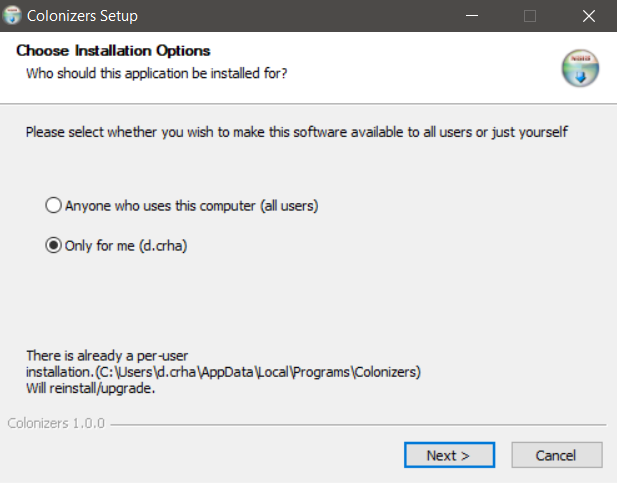
\includegraphics[width=110mm]{installer}}}
\caption{\emph{Colonizers} installer.}\label{ud:installer}
\end{figure}

The installer is an executable named \texttt{Colonizers Setup $x$.$y$.$z$.exe},
where $x$, $y$ and $z$ are placeholders for application versions. During installation,
the user will be asked whether they wish to install the application only for themselves,
or for all users of the computer. We recommend installing the application
only for the current user, since it does not require elevation. The installer
also allows the user to configure the installation directory,
as shown in \Cref{ud:installpath}.

\begin{figure}[ht]
\centerline{\mbox{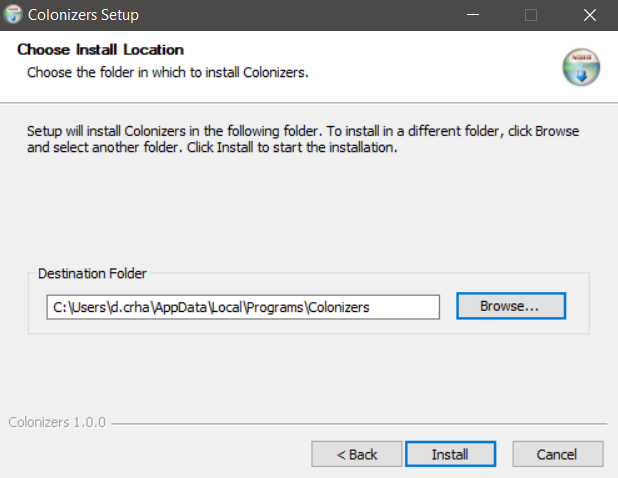
\includegraphics[width=110mm]{installpath}}}
\caption{Choosing the installation path in the installer.}\label{ud:installpath}
\end{figure}

When the installation is finished, the application may be launched from the specified
directory. The installer also adds \emph{Colonizers} into the Start menu, and creates
a~desktop shortcut for the game.

\subsection{Game Configuration}

After launching \emph{Colonizers}, the user will be presented with a~configuration
screen. On this screen, it is possible to configure the game and AI.

The first notable portion of this screen is the player selection, as shown
in \Cref{ud:playerselect}.

\begin{figure}[ht]
\centerline{\mbox{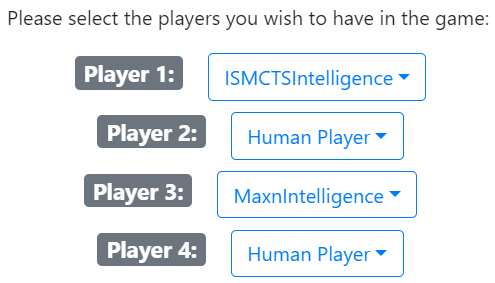
\includegraphics[width=110mm]{playerselect}}}
\caption{Player selection.}\label{ud:playerselect}
\end{figure}

This section contains four dropdowns, each
corresponding to a~player. Each dropdown lists all the available AIs
which are present in the user's game installation. By default, these dropdowns
will have the following values:
\begin{itemize}
    \item \texttt{Human Player}
    \item \texttt{HeuristicIntelligence}
    \item \texttt{ISMCTSIntelligence}
    \item \texttt{MaxnIntelligence}
    \item \texttt{RandomIntelligence}
\end{itemize}
\texttt{Human Player} means that on this player's turn, the UI will become interactible
and the user must choose action to perform. The other player options are AIs which
are bundled with the game. \Cref{ud:aicomp} shows a comparison of the aforementioned
AIs, based on the result of this thesis' experiments. Based on this table,
the user can choose the AI opponents which suit their needs.

\begin{table}[ht]
\centering
\begin{tabular}{l@{\hspace{1.5cm}} c c c c}
\textbf{AI} & \textbf{Strength} & \textbf{Evaluation speed} \\
\midrule
\texttt{RandomIntelligence}      & Weak   & Fast   \\
\texttt{HeuristicIntelligence}   & Moderate   & Fast  \\
\texttt{MaxnIntelligence}        & Moderate   & Moderate  \\
\texttt{ISMCTSIntelligence}      & Strong   & Slow   \\
\bottomrule
\end{tabular}
\caption{Simplified AI comparison.}\label{ud:aicomp}
\end{table}

There is an option to not enable information hiding. Normally, certain information
would be hidden on the screen, since that information is hidden in the game.
However, for purposes of testing AI, the option shown by \Cref{ud:hiddeninfo} can
be left unchecked. This will reveal all hidden information in the UI.
Note that this option does not affect the AI in any way, this option
is purely a~cosmetic one.

\begin{figure}[ht]
\centerline{\mbox{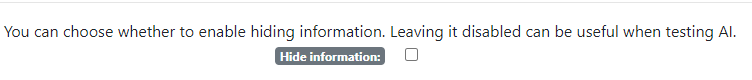
\includegraphics[width=110mm]{hiddeninfo}}}
\caption{Checkbox for hiding information.}\label{ud:hiddeninfo}
\end{figure}

The next section of configuration is are the buttons for adding new AI
into the game, as shown in \Cref{ud:aiaddbuttons}.

\begin{figure}[ht]
\centerline{\mbox{
\includegraphics[width=110mm]{aiaddbuttons}}}
\caption{Buttons for adding new AI scripts.}\label{ud:aiaddbuttons}
\end{figure}

These buttons open file select dialogs, allowing the user to add new AIs.
When adding an AI script, the script must follow the naming convention
of \texttt{<Name>Intelligence.py}, for example \texttt{CleverIntelligence.py}
\footnote{If an~AI is added this way which shares a~name with and existing AI,
the existing AI will be replaced by the new one. This also applies to AIs which
are bundled with the game}.
If the selected file does not follow this convention, it will not be recognized
by the game.
When adding an AI folder, the folder must follow the naming convention of
\texttt{<Name>Intelligence}, and this folder must contain a \texttt{main.py}
script. If the folder does not follow these conventions, it will not be recognized
by the game. This is explained in more depth in \Cref{chap:aidev}.

Lastly, this screen allows the configuration of the Python executable used
to execute AI scripts, as seen in \Cref{ud:pythonselect}. The shown
button will open a file select dialog, where the user can select their
installed Python executable.

\begin{figure}[ht]
\centerline{\mbox{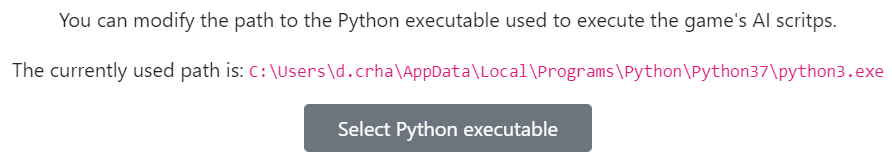
\includegraphics[width=110mm]{pythonselect}}}
\caption{Configuration of Python executable.}\label{ud:pythonselect}
\end{figure}

After the user is done configuring the game, they may start a game by clicking the
\emph{START GAME} button. Note that this button is disabled if the user
has not specified a Python executable to use.

\subsection{Gameplay}
\subsubsection{Board Overview}

After launching the game, the user will be greeted with a~view similar to
the one depicted in \Cref{ud:overview}.

\begin{figure}[ht]
\centerline{\mbox{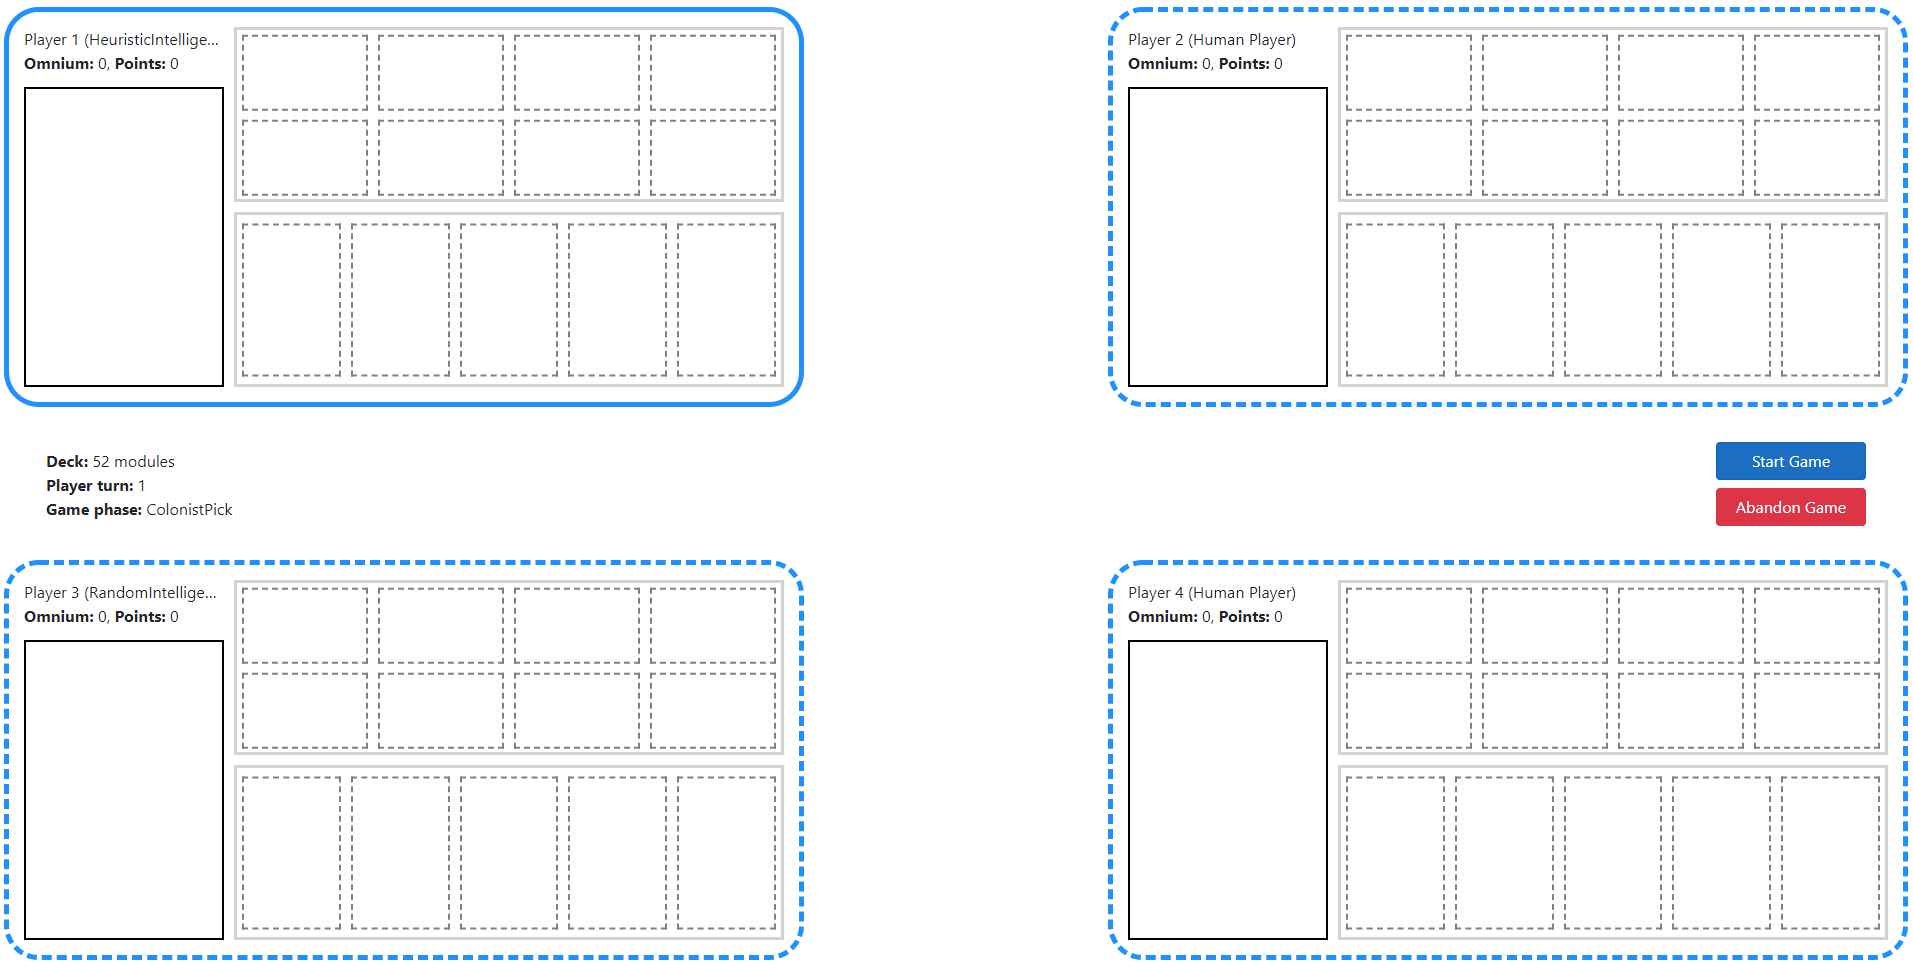
\includegraphics[width=130mm]{overview}}}
\caption{Overview of main game screen.}\label{ud:overview}
\end{figure}

This is the main game screen, and it is where all gameplay will be happening.
First off, we can focus on the buttons to the right of the screen, as shown in
\Cref{ud:buttons}.

\begin{figure}[ht]
\centerline{\mbox{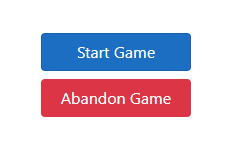
\includegraphics[width=60mm]{buttons}}}
\caption{Game control buttons.}\label{ud:buttons}
\end{figure}

These buttons control the flow of the game. The game does not start until the user
presses the \emph{Start Game} button. When the user does press it, the game starts
and the buttons becomes disabled. The other button, \emph{Abandon Game}, may be
pressed at any time during gameplay to immediately end the current game and return
to the configuration screen.

On the left side of the screen, we can also see micellaneous information about the
game state written in plain text. This information includes the amount of modules
left in the deck, the player on turn, and the current game phase.

The player overview areas are a core part of gameplay, you can see an example
of this area in \Cref{ud:player}.

\begin{figure}[ht]
\centerline{\mbox{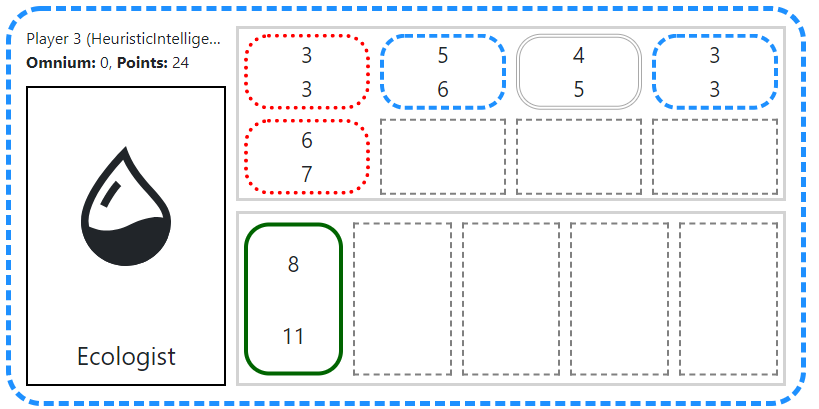
\includegraphics[width=110mm]{player}}}
\caption{Player overview.}\label{ud:player}
\end{figure}

This area contains all information about a given player. In the top left,
it shows the player's position and their name (meaning either \emph{Human Player},
or the name of the AI playing this player). In the top left we can also see
the amount of Omnium the player has (the game's currency) and the number of points
the player has the number of points determines the ranking at the end of the game.

On the left side of the player overview is the player's colonist card. This shows
the colonist this player has selected. A~colonist is a~character controlled
by the player for a~single turn, and the colonist provides the player with
special abilities to use at specific times of the game. The colonist is
easily identifiable by the icon and large text below it. For a~full description
of what abilities colonists have, please refer to \Cref{gamedesign:colonists}.

It is possible for this colonist card to be hidden, instead displaying a~card
featuring a large question mark. This can happen when hidden information is enabled
during game configuration. Specifically, a~player can only see another player's
colonist if the other player has already taken their turn.

Another feature shown by \Cref{ud:player} is the colony overview, seen in
\Cref{ud:colony}. This area contains the modules the player has built during
the game. The colony area has eight possible slots to build on. A square with
a grey dashed border is an empty slot. When any player
builds eight modules in their colony, the game will end at the end of the round,
after all players have taken their turn.

\begin{figure}[ht]
\centerline{\mbox{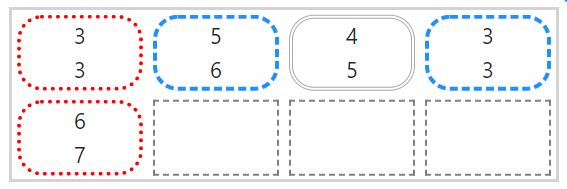
\includegraphics[width=110mm]{colony}}}
\caption{The colony overview.}\label{ud:colony}
\end{figure}

The elements with colored borders and two numbers inside them are called modules.
They are drawn by players from the deck, and they can be built in a~player's colony.
In order to build a module, the player must pay its build cost. A~module's build cost
is the number shown in the upper part of the module. When build in a~player's colony,
modules count towards that player's score. A~module's contribution to a player's
score is the number found in the bottom part of the module. Modules also have
a~color, depicted by the colored border \footnote{In order for the game to be accessible
to colorblind persons, the borders are also distinguished by the border pattern. A solid
line means green, a dashed line means blue, a dotted line means red, and a double line means
a module without a color.}
. This color is relevant during interactions
with certain colonist abilities. The modules in a player's colony are not hidden, and
are visible to other players even when information hiding is enabled.

The player overview seen in \Cref{ud:player} also contains the player's hand, as seen
in \Cref{ud:hand}.

\begin{figure}[ht]
\centerline{\mbox{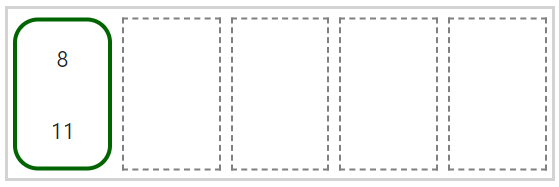
\includegraphics[width=110mm]{playerhand}}}
\caption{A player's hand.}\label{ud:hand}
\end{figure}

Whenever a player draws modules from the deck, they go into their hand. They then remain in
their hand until they are built, or removed by other means. The hand has a size limit of
five, it is not possible to draw more modules when a~player is at five modules in hand.
The modules in other players' hands are among the parts of the game board affected
by information hiding. If information hiding is enabled, modules in the hands of other
players will be displayed without color, and with question marks instead of
their real values.

The last feature of the player overview is its blue border. In \Cref{ud:player},
this border is dashed, meaning it is currently another player's turn. The player on
turn always has a~solid border around their player overview.

\subsubsection{Taking Turns}

Firstly, it should be noted that AIs take turns autonomously without any need of input
from the user. Whenever the turn is passed to an AI, it will immediately start
looking for the best move, and as soon as that move is found, it is played and the game
continues. This means that with AIs that make decisions particularly fast, if the game
is configured to have four of these AIs, the game can potentially end in mere seconds.
Therefore we will be discussing only features related to human players taking turns
for the rest of this section.

The first phase of a turn is the colonist pick phase. If you set up a game where
the first position has a human player, you will immediately be greeted with a selection
similar to the one seen in \Cref{ud:colonistpick}.

\begin{figure}[ht]
\centerline{\mbox{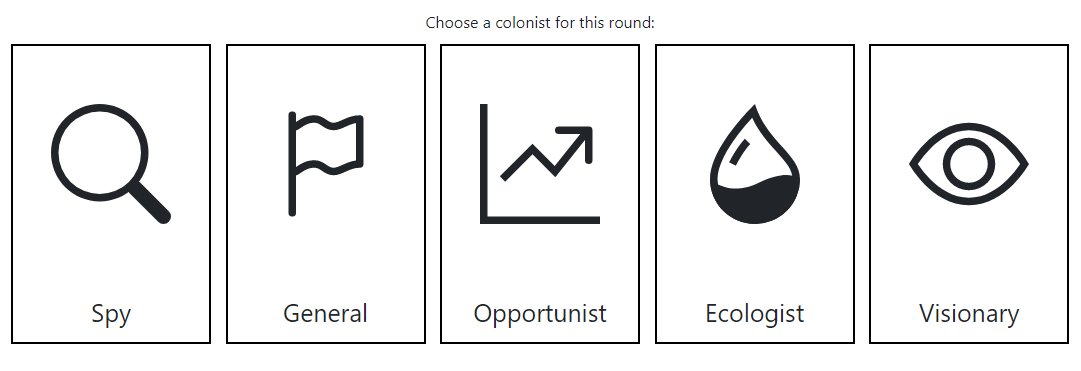
\includegraphics[width=130mm]{colonistpick}}}
\caption{Colonist selection.}\label{ud:colonistpick}
\end{figure}

At the start of each round, all players will take turns picking a colonist,
in order of first player to last. Note that only five out of the total
six are available for selection at any given time, since one is randomly removed
from play every round. Selecting a colonist is done by clicking on the corresponding
colonist card.

After all players have picked their colonist, players will each take their turn,
in order from first to last. The first phase of a player's individual turn is
the draw phase, as seen in \Cref{ud:drawphase}. The shown buttons will be present
in a card overlaying the game board, similarly to the colonist pick phase.
Colonist passive abilities trigger automatically during the draw phase.

\begin{figure}[ht]
\centerline{\mbox{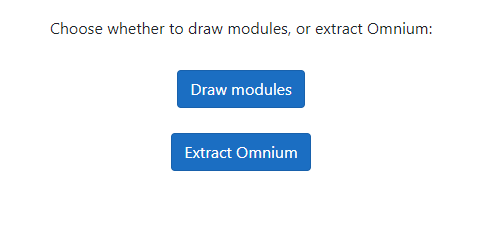
\includegraphics[width=110mm]{drawphase}}}
\caption{Draw phase selection.}\label{ud:drawphase}
\end{figure}

At this point, a player may choose to either gain two Omnium, order
draw two modules from the deck and discard one of them.
Note that the draw action will be unavailable if the player's hand is full.
If the player chooses to draw modules, they will be presented with an additional
dialog as seen in \Cref{ud:discardphase}. The player must choose which module they
want to keep, and which they want to discard. The choice is made by clicking on the
module the player wishes to keep.

\begin{figure}[ht]
\centerline{\mbox{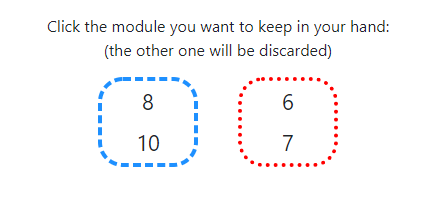
\includegraphics[width=110mm]{discardphase}}}
\caption{Choice of module to discard.}\label{ud:discardphase}
\end{figure}

The next phase is the colonist power phase. If the player control a~colonist
with an~active ability (Opportunist or Spy), they will be presented with a~choice
similar to that shown in \Cref{ud:powertarget}. The player may choose to target
a given colonist by clicking on their respective card, or the player may choose
to not use their colonist's ability by clicking the \emph{Do nothing} button
to the right.

\begin{figure}[ht]
\centerline{\mbox{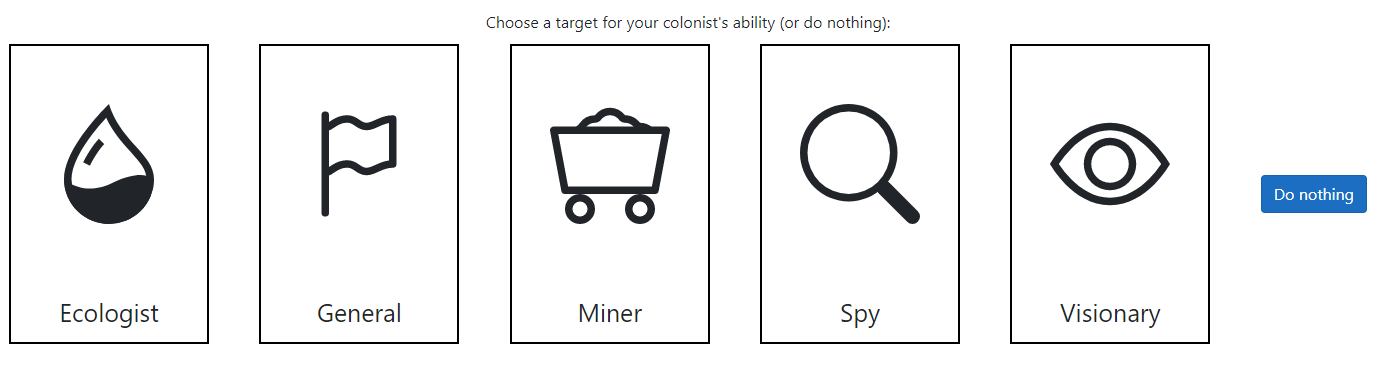
\includegraphics[width=130mm]{powertarget}}}
\caption{Selection of colonist active ability target.}\label{ud:powertarget}
\end{figure}

Players controlling colonists without active abilities will instead be presented
with a small dialog containing a single button which passes the phase.

The last phase of a turn is the build phase. In this phase, players may build
up to one module from their hand by spending the required amount of Omnium.
Modules which the player can afford to build will have a hammer icon present.
Clicking this icon will build the module in the player's colony. If the hammer
icon is not present, it means that the player cannot afford the module,
or the game is not in the build phase. The hammer icon is shown in
\Cref{ud:buildhammer}, next to a module without the hammer icon.

\begin{figure}[ht]
\centerline{\mbox{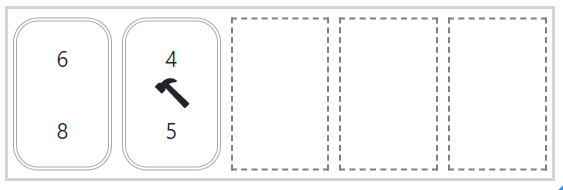
\includegraphics[width=110mm]{buildhammer}}}
\caption{Hammer icon used to build modules from the hand.}\label{ud:buildhammer}
\end{figure}

After all players end their turns, the round will end and a new round will begin,
starting again with the colonist pick phase. New rounds will keep
starting after the previous round ends until a player has built eight
modules in their colony. The first player to reach eight modules receives
four bonus point on game end, and subsequent players to reach eight modules
receive two points each. When the game ends, a dialog will open showing the user
the final ranking and final scores. This final score table is shown in
\Cref{ud:gameover}.

\begin{figure}[ht]
\centerline{\mbox{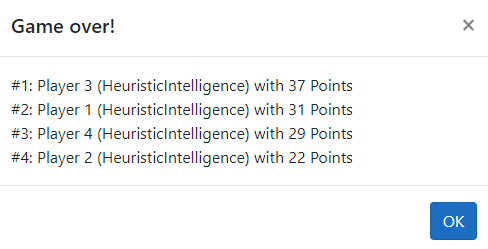
\includegraphics[width=110mm]{gameover}}}
\caption{Game over screen with final scores.}\label{ud:gameover}
\end{figure}

Here, the player may either click \emph{OK} to go back to the game configuration
screen, or they may simply close the dialog and spend time looking at the final
game board state. When the user wishes to return to the game configuration screen,
they may press the \emph{Abandon Game} button to do so.

\clearpage

\pagebreak
\section{Developer Documentation}
\label{sec:devdocs} 

\subsection{Prerequisites}

In order to do development work on \emph{Colonizers}, the following software
is required:
\begin{itemize}
    \item .NET Core 3.1 SDK
    \item Python 3.7
    \item Node.js 10 and NPM 6.4.1
\end{itemize}
The game's UI is designed for a minimum screen resolution of 1920x1080 at
100\% zoom level. It is not recommended to play the game on lower resolution
screens, since graphical errors may occur.

In order to build and run \emph{Colonizers} in Electron, the Electron.NET CLI
package is required. You may install this package as a .NET Core tool by running
the \texttt{dotnet tool install ElectronNET.CLI -g} command. This gives you
access to the \texttt{electronize} command.

It is also highly recommended to use Visual Studio 2019 for development work
on the game engine or the UI. Visual Studio 2019 provides support for debugging
both the UI and the game engine in the same window, which makes for a~seamless
development experience. Visual Studio 2019 is also capable of attaching
to an external process for debugging, which turns out to be
extremely useful with Electron.NET.

For developing and debugging Python AI scripts, the author used Visual Studio Code,
but other software capable of debugging Python scripts is viable as well.

\subsection{Project Structure}

The entire game is contained in a .sln (solution) file, which is a file type used
to organize projects in Visual Studio. This solution contains four projects:
\begin{itemize}
    \item \texttt{AICore} --- project with the API for AI scripts and the AICore
        scripts themselves.
    \item \texttt{Desktop} --- project with the UI, consisting of an~Angular
        web application and an ASP.NET Core Web API. The Web API is the
        \emph{ClientApp} subfolder of this project's folder.
    \item \texttt{Game} --- C\# library project containing the game logic
        and code responsible for communicating with Python AIs.
    \item \texttt{Experiments} --- console application project containing
        the experiment scenarios explored in this thesis.
\end{itemize}

The flow of data in the application starts with the UI, since all initiative starts
with the user. The UI then uses the ASP.NET Core Web API to execute game logic.
If required, game logic then talks to processes executing Python AI sripts.
This flow can be seen in \Cref{dd:sequence}.

\begin{figure}[ht]
\centerline{\mbox{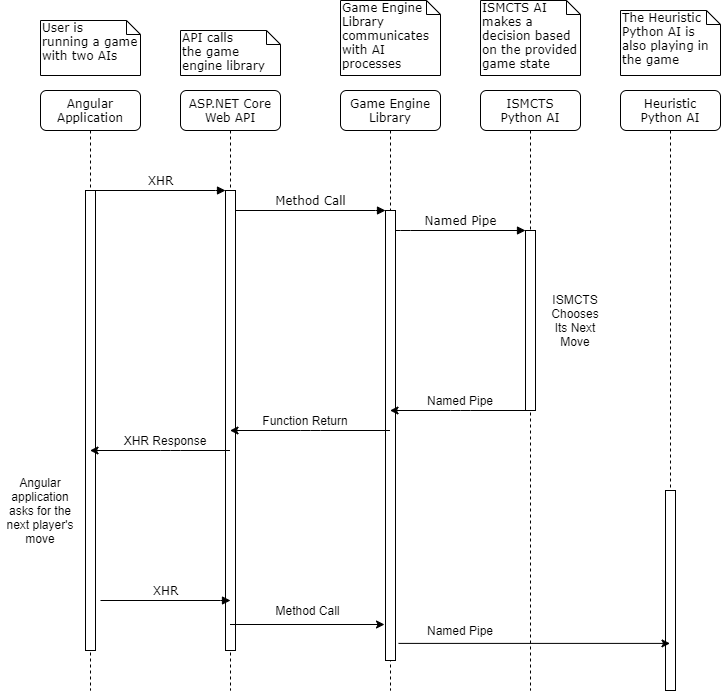
\includegraphics[width=130mm]{colonizers-sequence}}}
\caption{\emph{Colonizers} sequence diagram.}\label{dd:sequence}
\end{figure}

The aforementioned components will be discussed in more detail in the following subsections.

\subsection{Game Engine}

WORK IN PROGRESS

\subsection{Artificial Intelligence}
\label{chap:aidev}

WORK IN PROGRESS

\subsection{User Interface}

\emph{Colonizers} uses Electron as a means to run the game as a desktop application,
since the game is developed using web technologies. Specifically, it uses the
Electron.NET library, which provides an access to the Electron APIs to C\# applications,
and it also facilitates usage of Electron's build tools to package C\# applications.
C\# and the whole .NET platform in general still do not have a widely-used cross-platform
UI framework, therefore Electron was a good fit for this project.

The UI for \emph{Colonizers} is an Angular application, which is then served inside
Electron. Electron then uses the Chromium rendering engine and Node.js in the background.
The Angular application allows configuration of the game, it handles presentation
of game state to the user, and it is responsible for communicating with the
ASP.NET Core Web API.

In order to do development work on the UI, it is recommended that you use
Visual Studio 2019. It has a very useful feature whereby it allows you to debug
both JavaScript and C\# code at the same time in the same project. Since the Angular
application is located in the same project as the Web API, this is an invaluable
feature. Since the UI is an Angular application, naturally it is possible
to run and debug it without running it in Electron. The source code for this project
contains launch settings pre-configured for Visual Studio 2019 in order to accomplish
exactly this. A sidenote is that while running outside Electron, the application
does not have access to Electron APIs. \emph{Colonizers} uses the File Dialog
API multiple times, therefore this functionality will be unavaliable in this case.
Interaction with the Electron APIs is always preceded by a check whether
the application instance is running inside Electron, therefore calls
to methods which use Electron APIs will not cause exceptions. We can see
such a guard for Electron presence in \Cref{dd:electronguard}.

\begin{figure}[hb]
\begin{code}[commandchars=\\\{\},codes={\catcode`\$=3\catcode`\^=7\catcode`\_=8}]
public async Task<bool> AddSingleScript()
$\{$
    if (HybridSupport.IsElectronActive)
    $\{$
        BrowserWindow mainWindow = Electron.WindowManager
            .BrowserWindows.First();
        OpenDialogOptions options = new OpenDialogOptions
        $\{$
            Properties = new OpenDialogProperty[] $\{$
                    openDialogProperty
                $\}$
        $\}$;

        string[] files = await Electron.Dialog.ShowOpenDialogAsync(
            mainWindow, options);
    $\}$

    return false;
$\}$
\end{code}
\caption{Electron API call guarded by check for Electron presence.}\label{dd:electronguard}
\end{figure}

The source code for the Angular application is written in TypeScript, CSS and HTML.
The HTML used is not pure HTML, rather the HTML files are Angular templates.
Angular Templates are a way to insert data into markup seamlessly.
The TypeScript files are transpiled to JavaScript at build-time.

The most important building blocks of Angular are \emph{Components}.
Components control the view presented to the user, and they prepare
data for presentation by the view. We can see the source code for a component
in \Cref{dd:componentcode}

\begin{figure}[ht]
\begin{code}[commandchars=\\\{\},codes={\catcode`\$=3\catcode`\^=7\catcode`\_=8}]
@Component($\{$
    selector: 'app-discard',
    templateUrl: './discard.component.html',
    styleUrls: ['./discard.component.css']
$\}$)
export class DiscardComponent implements OnInit $\{$

    @Input() gameState: GameState;
    @Output() onPick = new EventEmitter<number>();

    constructor() $\{$ $\}$

    ngOnInit() $\{$
    $\}$

    getModules(): Module[] $\{$
        // Find the appropriate modules in the temp discard storage
        return this.gameState.actions.map(
            x => this.gameState.boardState.discardTempStorage
                .find(y => y.name === x.module));
    $\}$

    keep(module: Module) $\{$
        this.onPick.next(this.gameState.actions.findIndex(
            x => x.module == module.name));
    $\}$

$\}$
\end{code}
\caption{An Angular component.}\label{dd:componentcode}
\end{figure}

We can see a few important component features in \Cref{dd:componentcode}:
\begin{itemize}
    \item The definition of the component's template and styles
        in the \texttt{@Component} decorator. Notably, the styles
        specified in this scope only apply to this component's
        template.
    \item The component has an \texttt{@Input()} and an \texttt{@Output()}.
        These are the ways other components interact with this one.
        Keeping component interaction to only inputs and outputs makes
        components pure, meaning they will output the same data
        when provided with the same inputs. In a complex application,
        this is a very desirable property, since it makes debugging
        easier and bugs more rare.
    \item The component defines a selector --- \texttt{app-discard}.
        Using this selector, other components can include this one in
        their templates.
\end{itemize}

We can see an example of the aforementioned component being used in \Cref{dd:componentref}.
The excerpt is from \texttt{GameComponent}'s template, and it demonstrates how
it binds one of its own fields as an input for the \texttt{DiscardComponent},
and that it is listening for events emitted by it.

\begin{figure}[ht]
\begin{code}[commandchars=\\\{\},codes={\catcode`\$=3\catcode`\^=7\catcode`\_=8}]
<div *ngIf="isWaitingForHumanPlayer && isDiscardPhase()">
    <app-discard [gameState]="gameState"
                 (onPick)="onHumanPlayerAction(\$event)">
    </app-discard>
</div>
\end{code}
\caption{Usage of Angular component in another component's template.}\label{dd:componentref}
\end{figure}

These features are the core of how the UI application is built --- it is based on
a~divide-and-conquer principle, where the entire view is composed of smaller components,
which are in turn composed of even smaller components. 

\clearpage
\subsection{Experiments}
\label{chap:experimentdocs}

The experiments performed in this thesis are implemented in the \texttt{Experiments}
project of the \texttt{Colonizers} solution. It is a C\# console application project.
It is invoked via the command line with two arguments --- the first is a~number
between 1 and 5, corresponding to the experiment number, and the second
is the path to the Python executable to use when executing AI scripts.

% TODO: verify where the JSON file is generated
After the experiment is run, it will produce a JSON file containing the results
of the experiment. This file is generated in the directory where the experiments
are running.
\Cref{dd:experimentjson} shows the structure of these JSON files, with less
important fields omitted for brevity. The JSON files associated with the five
experiments are also located in the \texttt{Experiments} projects, namely in
the \texttt{Results} folder. They were added there for reference, since
some experiments may take tens of hours to run even on reasonably fast
machines. Be aware that a simple diff of the JSON result files
is not sufficient for determining whether or not a given experiment was successfully
replicated. This is because the files contain running times of the games as well.

\begin{figure}[ht]
\begin{code}[commandchars=\\\{\},codes={\catcode`\$=3\catcode`\^=7\catcode`\_=8}]
$\{$
    "Players": [
        "Name": "ISMCTS",
        "PlayerEndInfo": $\{$
            "Ranking": 3,
            "VictoryPoints": 24,
            "Player": $\{$
                "ID": 1,
                ...
            $\}$
        $\}$
    ],
    "Duration": "00:12:28.1879334"
$\}$
\end{code}
\caption{Experiment result JSON file structure (simplified).}\label{dd:experimentjson}
\end{figure}

The class \texttt{Scenarios} contains the setup for the experiments,
and each scenario then calls \texttt{ExperimentRunner} to performed
the experiment itself.

A noteworthy point is the implementation of the shuffling of players between games.
Since the game engine already possessed an implementation of the Fisher-Yates Shuffle
\cite{Knuth98} for shuffling lists, this implementation was reused for shuffling the
players themselves. This means that if we were to run the experiments
without shuffling, and instead assigning the players the same positions they would
have been assigned by the shuffle, the results of this experiment would be different.
This is because running the shuffle manipulates the game engine's random number generator.


\openright
\end{document}
